% !TeX program = xelatex
\RequirePackage{fix-cm}
\documentclass[UTF8,a4paper,zihao=-4,fontset=fandol]{ctexart}
\usepackage[left=24mm,right=24mm,top=23mm,bottom=23mm]{geometry}
\usepackage{lmodern}
\usepackage{booktabs,tabularx,longtable,array,graphicx,xcolor,amsmath}
\usepackage{enumitem,caption,placeins,needspace,float,hyperref}
\hypersetup{unicode=true,hidelinks,pdftitle={EdgeSight 技术报告},pdfauthor={EdgeSight 团队}}
\urlstyle{same}
\graphicspath{{../figures/}}
\setlength{\parindent}{2em}
\setlength{\parskip}{0.3em}
\linespread{1.2}
\setlength{\emergencystretch}{2em}
\widowpenalty=10000
\clubpenalty=10000
\setcounter{tocdepth}{2}
\setcounter{topnumber}{4}
\setcounter{bottomnumber}{3}
\setcounter{totalnumber}{6}
\renewcommand{\topfraction}{0.95}
\renewcommand{\bottomfraction}{0.9}
\renewcommand{\textfraction}{0.05}
\renewcommand{\floatpagefraction}{0.7}
\makeatletter
\setlength{\@fptop}{0pt}
\setlength{\@fpsep}{18pt}
\makeatother
\setlist{nosep,leftmargin=2em}
\captionsetup{font=small,labelfont=bf,labelsep=quad}
\ctexset{section={format=\Large\bfseries},subsection={format=\large\bfseries},subsubsection={format=\normalsize\bfseries}}
\newcolumntype{Y}{>{\raggedright\arraybackslash}X}
\newcolumntype{P}[1]{>{\raggedright\arraybackslash}p{#1}}
\newcommand{\code}[1]{\texttt{\detokenize{#1}}}
\newcommand{\todo}{\textbf{待补充}}
\newcommand{\measure}{待实测}
\newcommand{\sourcepath}[2]{\href{https://github.com/never-die-cold/FPGA-Alittle-Design/blob/a631fd2/#1}{#2}}
\newcommand{\figplaceholder}[4]{%
  \begin{figure}[H]\centering
  \fbox{\parbox[c][#4][c]{0.88\linewidth}{\centering\small 图片占位\par\medskip #3\par\medskip 待补充}}
  \caption{#1}\label{#2}\end{figure}}
\begin{document}
\hypersetup{pageanchor=false}
\begin{titlepage}
\vspace*{18mm}
\noindent{\LARGE\bfseries EdgeSight（边缘慧眼）\par}
\vspace{7mm}
\noindent{\Large 基于自研 RISC-V 的边缘智能视觉 SoC 技术报告\par}
\vspace{13mm}
\noindent\begin{tabularx}{\linewidth}{@{}lY@{}}
\toprule
参赛方向 & AMD 自主选题赛道（初级组）\\
文档版本 & v0.1，提交初稿（LaTeX 版）\\
修订日期 & 2026 年 10 月 30 日\\
源码基线 & 分支 \code{dev/submission-slim}，提交 \code{a631fd2}\\
目标平台 & AMD PYNQ-Z2（XC7Z020-1CLG400C）\\
团队与成员 & \todo\\
\bottomrule
\end{tabularx}
\par\vspace{12mm}
\noindent\textbf{摘要}\par
EdgeSight 是面向受控工位紧固件识别与工业检查的边缘智能视觉系统。
系统在 PYNQ-Z2 的可编程逻辑内同时部署自研 RV32IM 处理器核、HDMI 视觉预处理流水线与 INT8 CNN 推理协处理器。
处理器核通过 44 项 RISC-V 架构测试签名，OOC 实点 86.806 MHz；SoC 以 40 MHz 上板。
视觉链路支持 720p60 显示直通与灰度分析分流。
协处理器整网推理 472,593 拍，板上输出与整数参考逐项一致。
本文依次说明作品概述、系统组成、三个自研模块、数据与工业闭环、完成情况与验证边界。
\vfill
\noindent\small 本文范围：当前源码实现的模块、已留档的实测结果，以及提交前所需的图片与未闭环清单。
\end{titlepage}
\hypersetup{pageanchor=true}
\begingroup
\small
\setlength{\parskip}{0pt}
\linespread{1}\selectfont
\tableofcontents
\endgroup
\clearpage
\Needspace{10\baselineskip}
\section{作品概述}
\label{sec:overview}

\subsection{功能与特性}
EdgeSight 面向受控工位的螺栓、螺母、垫圈识别与检查。
真实 HDMI 相机提供画面；板卡完成预处理、目标定位与分类；自研 RISC-V 核按工单汇总判定；PS 提供结果与配置通信；网页端展示视频、目标框、类别与检查结论。
首版功能包括按类别计数、工单核对（缺件、多余件、错料）、一次检查一条批次记录、异常截图与记录导出、设备连接与推理状态诊断。

\subsection{应用领域}
紧固件工业检查。
工位背景简单、稳定可控、照明理想；物体自由摆放且互不遮挡。
实际支持范围由采样验证，阴影、反光、接触与遮挡不在首版范围内，超条件时提示复检。

\subsection{主要技术特点}
三个自研数字模块共存于同一片可编程逻辑：RISC-V 处理器核、HDMI 视觉预处理流水线、INT8 CNN 推理协处理器。
接口以冻结契约为准；每一级实现都有仓库内的黄金参考与回归入口。
性能口径区分外推、实点与板上三档，不做无证据声明。

\subsection{主要性能指标}
表~\ref{tab:keymetrics} 汇总关键指标，每行标注口径日期；依据见对应参考文献。

\begin{table}[H]\centering\small
\caption{主要性能指标与口径}\label{tab:keymetrics}
\begin{tabularx}{\linewidth}{@{}P{30mm}Y P{20mm}@{}}\toprule
指标 & 数值与口径 & 日期\\\midrule
处理器核 & v1 三级流水、三路转发、Radix-4 乘除、可切换 BHT & 2026-09-27\\
CoreMark & CPI 1.886（无转发）$\rightarrow$ 1.606（转发+BHT2），retired 10{,}106{,}386 & 2026-10-07\\
架构测试 & riscv-arch-test I+M 子集 44/44 签名匹配 & 2026-10-07\\
核时序 & OOC 实点 86.806 MHz（BHT2 @ 11.52 ns，WNS +0.538 ns） & 2026-10-07\\
最小 SoC & 40 MHz 上板，LED 判据；LUT 6{,}768、BRAM 8、DSP 0 & 2026-10-07\\
视觉链路 & 720p60；\code{video_pipeline} OOC WNS +0.330 ns & 2026-10-27\\
协处理器 & 128 MAC INT8；整网 472{,}593 拍；DSP 136/220、BRAM36 69/140 & 2026-10-15\\
整机门禁 & WNS +2.078 ns（A 包，含协处理器） & 2026-10-27\\
板上 CNN & zero/pattern 各 3 轮 6/6 匹配；四例黄金全匹配 & 2026-10-26\\
多目标实板 & 12 轮 85 个结果与整数参考逐项一致（CNN r6） & 2026-10-28\\\bottomrule
\end{tabularx}\end{table}

\subsection{主要创新点}
在同一片 FPGA 内完成感知、推理与调度的全自研闭环：视觉预处理、INT8 协处理器与自研 RISC-V 核分工协作，不依赖第三方处理器软核。
建立契约先行与逐位黄金对拍的质量体系：量化网络、流水线时序与推理结果都有独立参考。
把大模型协作制度化为理解门槛与证据目录，AI 产出经讲解、答题与独立审查后才入库。

\subsection{设计流程}
设计按八阶段推进：需求与验收、接口契约、RTL 与模块 tb、全量回归、综合与时序、上板 bring-up、软件联调、证据归档（图~\ref{fig:flow}）。
每阶段以门禁与仓库内脚本收口；仿真、软件、板上三级别分别标注，不用低级别证据替代高级别结论。

\begin{figure}[H]\centering
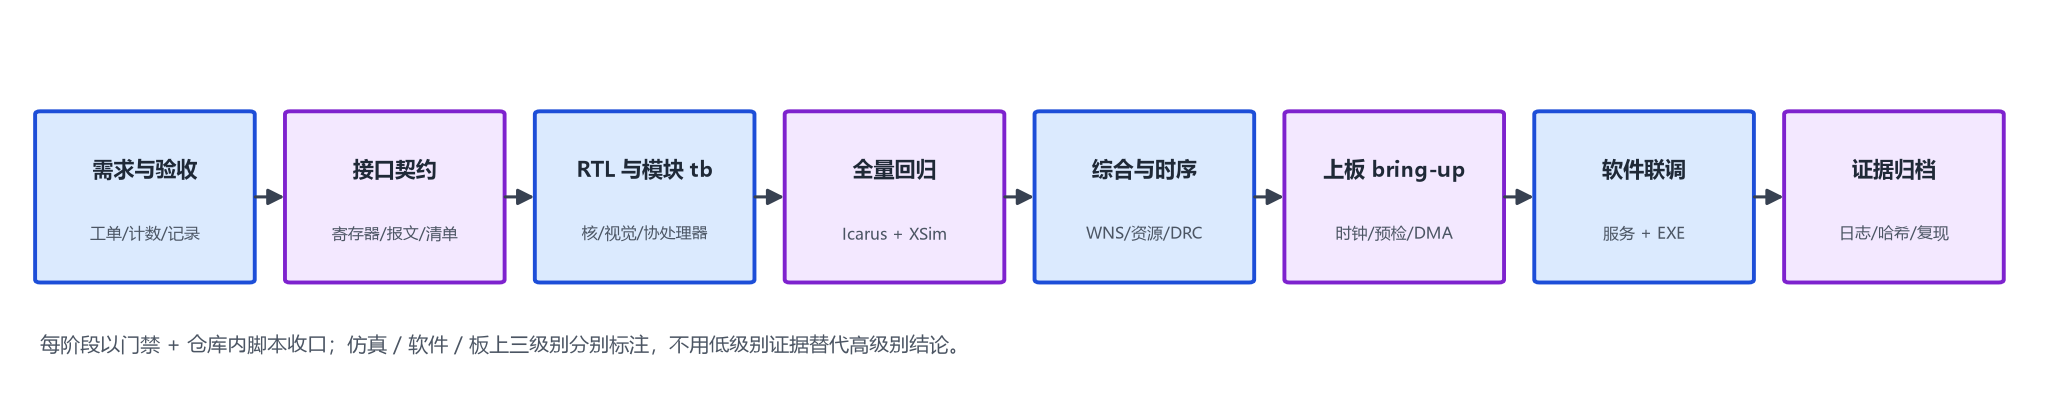
\includegraphics[width=0.98\linewidth]{fig_flow.png}
\caption{设计流程八阶段与门禁收口（仓库配图）}\label{fig:flow}
\end{figure}

\Needspace{10\baselineskip}
\section{系统组成与软硬件划分}
\label{sec:architecture}
系统由可编程逻辑（PL）的三个自研模块、处理系统（PS）的采集与服务、PC 浏览器前端组成。
总体架构与数据路径见图~\ref{fig:system}；模块划分见表~\ref{tab:components}。

\begin{figure}[H]\centering
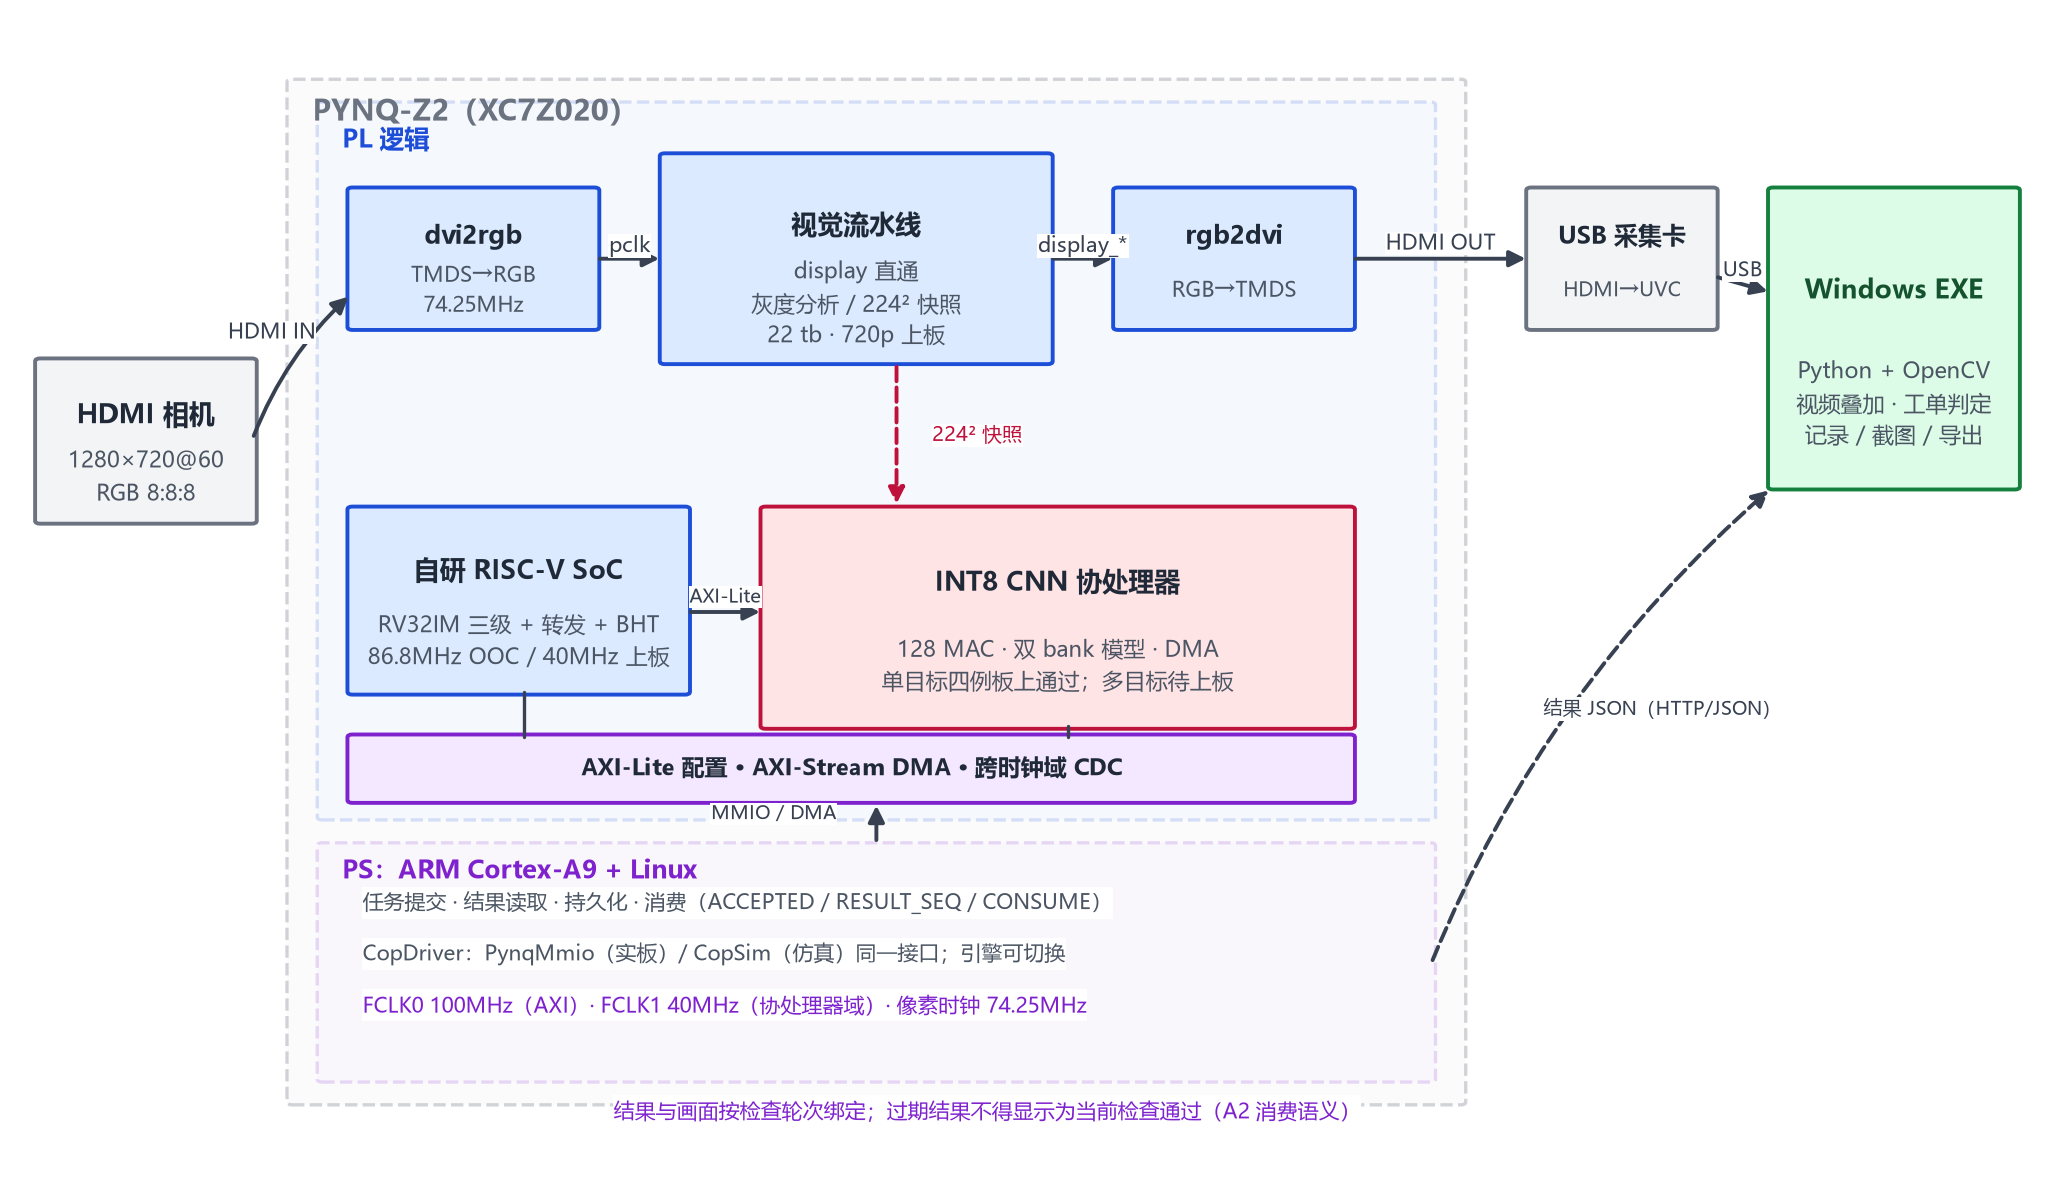
\includegraphics[width=0.98\linewidth]{fig_system.png}
\caption{系统总体架构与数据路径（仓库配图）}\label{fig:system}
\end{figure}

\begin{table}[H]\centering\small
\caption{模块划分与运行位置}\label{tab:components}
\begin{tabularx}{\linewidth}{@{}P{34mm}P{30mm}Y@{}}\toprule
模块 & 运行位置与实现 & 主要职责\\\midrule
视觉预处理流水线 & PL，Verilog-2001 & 对齐、滤波、缩放、缓存与显示直通\\
CNN 推理协处理器 & PL，Verilog-2001 & 64$\times$64 ROI 的 INT8 推理与结果寄存\\
自研 RISC-V 核 & PL，Verilog-2001 & 检查调度、数量汇总与工单判定\\
目标定位与 ROI & PS，Python（OpenCV） & 连通域定位、外接框与 64$\times$64 裁剪\\
板端服务 & PS，Python & park 取帧、LIVE API、轮次关联与记录\\
网页前端 & PC 浏览器，HTML & 视频叠加、交互、统计展示与导出\\\bottomrule
\end{tabularx}\end{table}

\subsection{视频与分析数据流}
相机画面经 HDMI 输入进入预处理流水线。
彩色原图以恒定延迟直通 \code{display_*} 口输出 HDMI OUT，板上显示保留彩色原图。
分析路径在 PL 内有独立的灰度 \code{out_*} 口（模块级实现，含滤波与缩放）；现役共存位流未接入该支路，
板端直接捕获 native RGB/BGR 原帧，由 PS 用 OpenCV 定位并裁剪出 64$\times$64 灰度 ROI，交给协处理器推理。
结果槽经轮次协议关联后进入网页端；\code{out_*} 口的框叠加只作诊断，不代表物体定位。
视频与分析的关联采用冻结的轮次协议 v1.2：判据为 \code{session_id}、\code{config_id} 与年龄窗口，\code{frame_id} 仅透传；过期、断联或无法确认的画面不得显示为当前检查通过。

\subsection{软硬件责任边界}
表~\ref{tab:boundary} 按冻结契约列出责任边界；契约编号见附录术语表。

\begin{table}[H]\centering\small
\caption{软硬件责任边界（C03 分工口径）}\label{tab:boundary}
\begin{tabularx}{\linewidth}{@{}P{40mm}Y@{}}\toprule
事务 & 责任方\\\midrule
视频预处理与显示 & PL 视觉流水线\\
目标定位与 ROI 裁剪 & PS（OpenCV；C03 冻结项，后续下沉 PL 需另评审）\\
CNN 推理 & PL 协处理器（C02 整数契约）\\
检查调度与工单判定 & 自研 RISC-V 核固件（C03 分工）\\
结果通信与配置 & PS 服务（轮次协议 v1.2，16 目标能力上限）\\
展示、交互与记录 & 网页端（检查记录 v2 与 CSV 导出）\\\bottomrule
\end{tabularx}\end{table}

\subsection{演示链路}
演示链路为相机 HDMI 输出接入板卡 HDMI IN，HDMI OUT 经 USB 采集卡回显至 PC，检查结果经网口同步至浏览器网页端（实物布置见图~\ref{fig:photo}）。
采集卡延迟为采集链路自身参数，不计入板端处理指标。

\begin{figure}[H]\centering
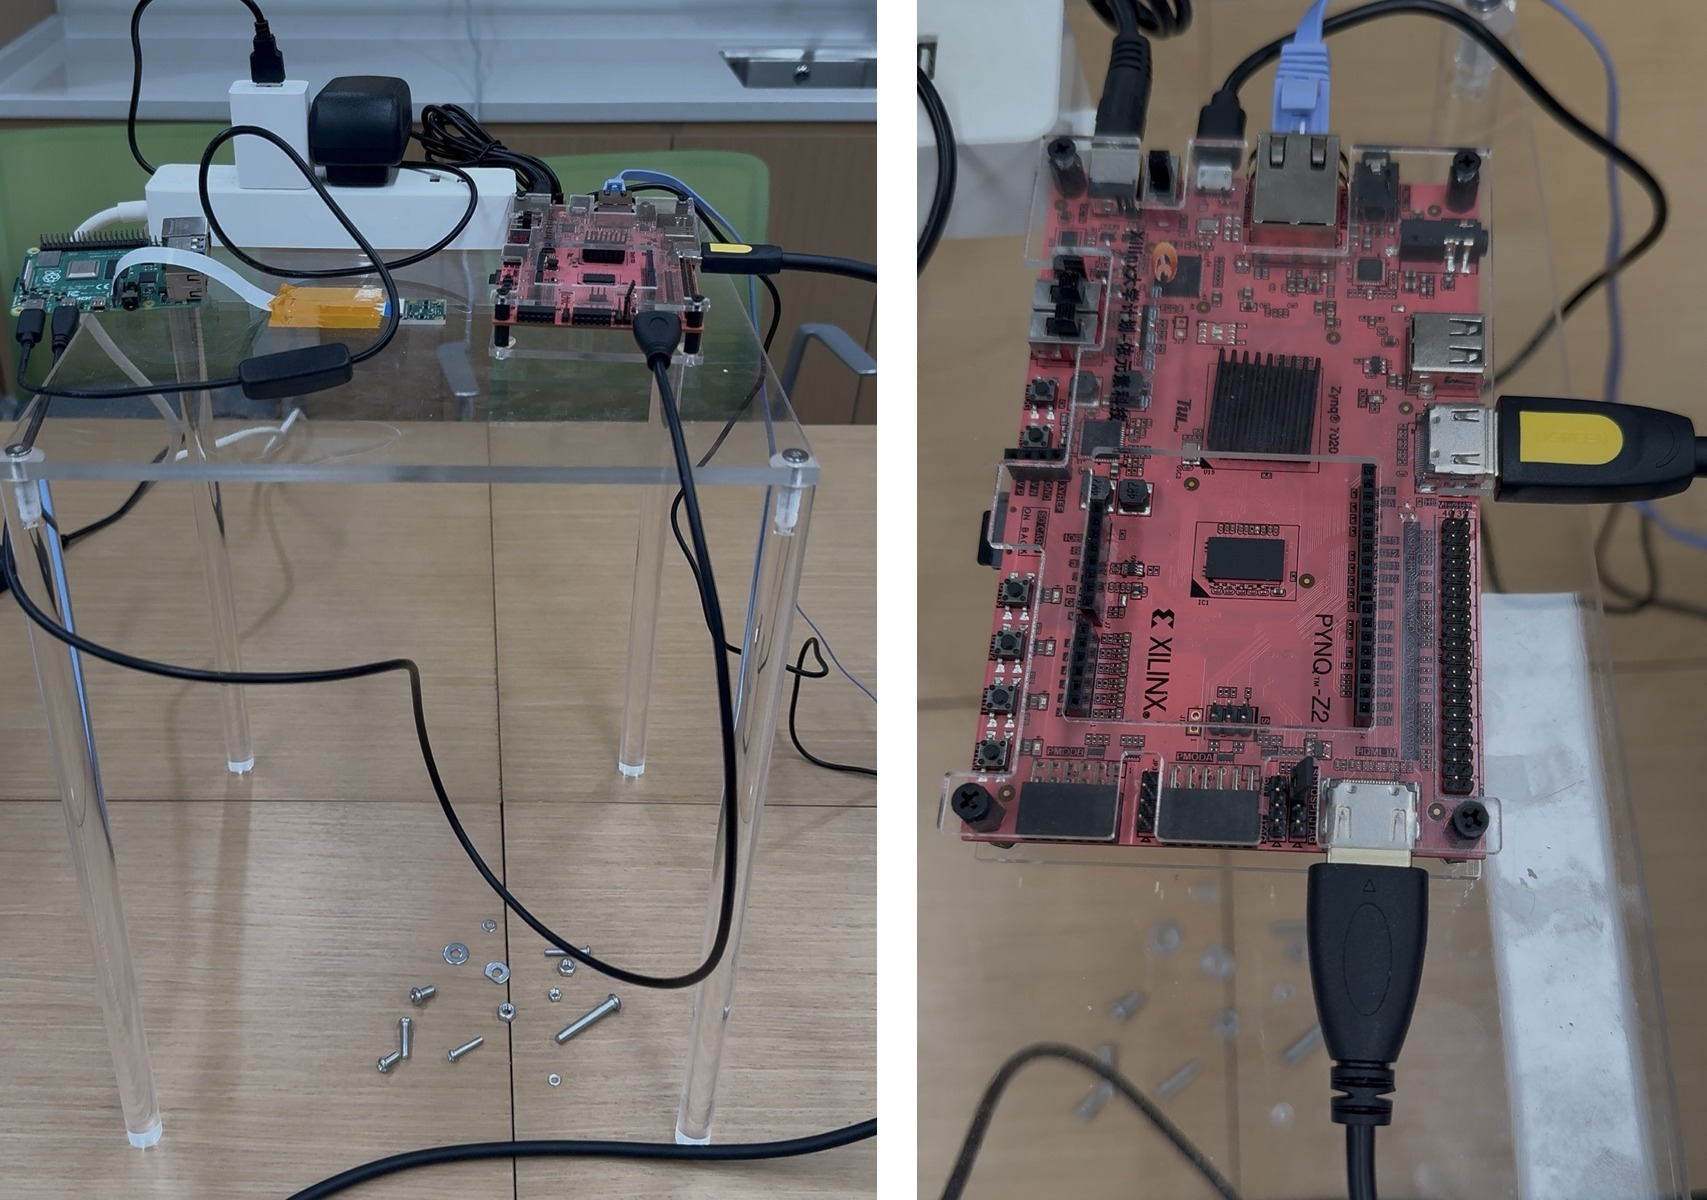
\includegraphics[width=0.9\linewidth]{photo_plate.jpg}
\caption{实物布置与 PYNQ-Z2 板卡接线（仓库照片）}\label{fig:photo}
\end{figure}
\FloatBarrier

\clearpage
\Needspace{10\baselineskip}
\section{自研 RISC-V 处理器核}
\label{sec:core}
处理器核为自研 RV32IM 实现，v0 两级流水基线，v1 升级为三级流水并加入转发与分支预测。
微架构见图~\ref{fig:core}。
接口契约以 \code{design_v0.md} 与 \code{design_v1.md} 冻结版本为准。

\begin{figure}[H]\centering
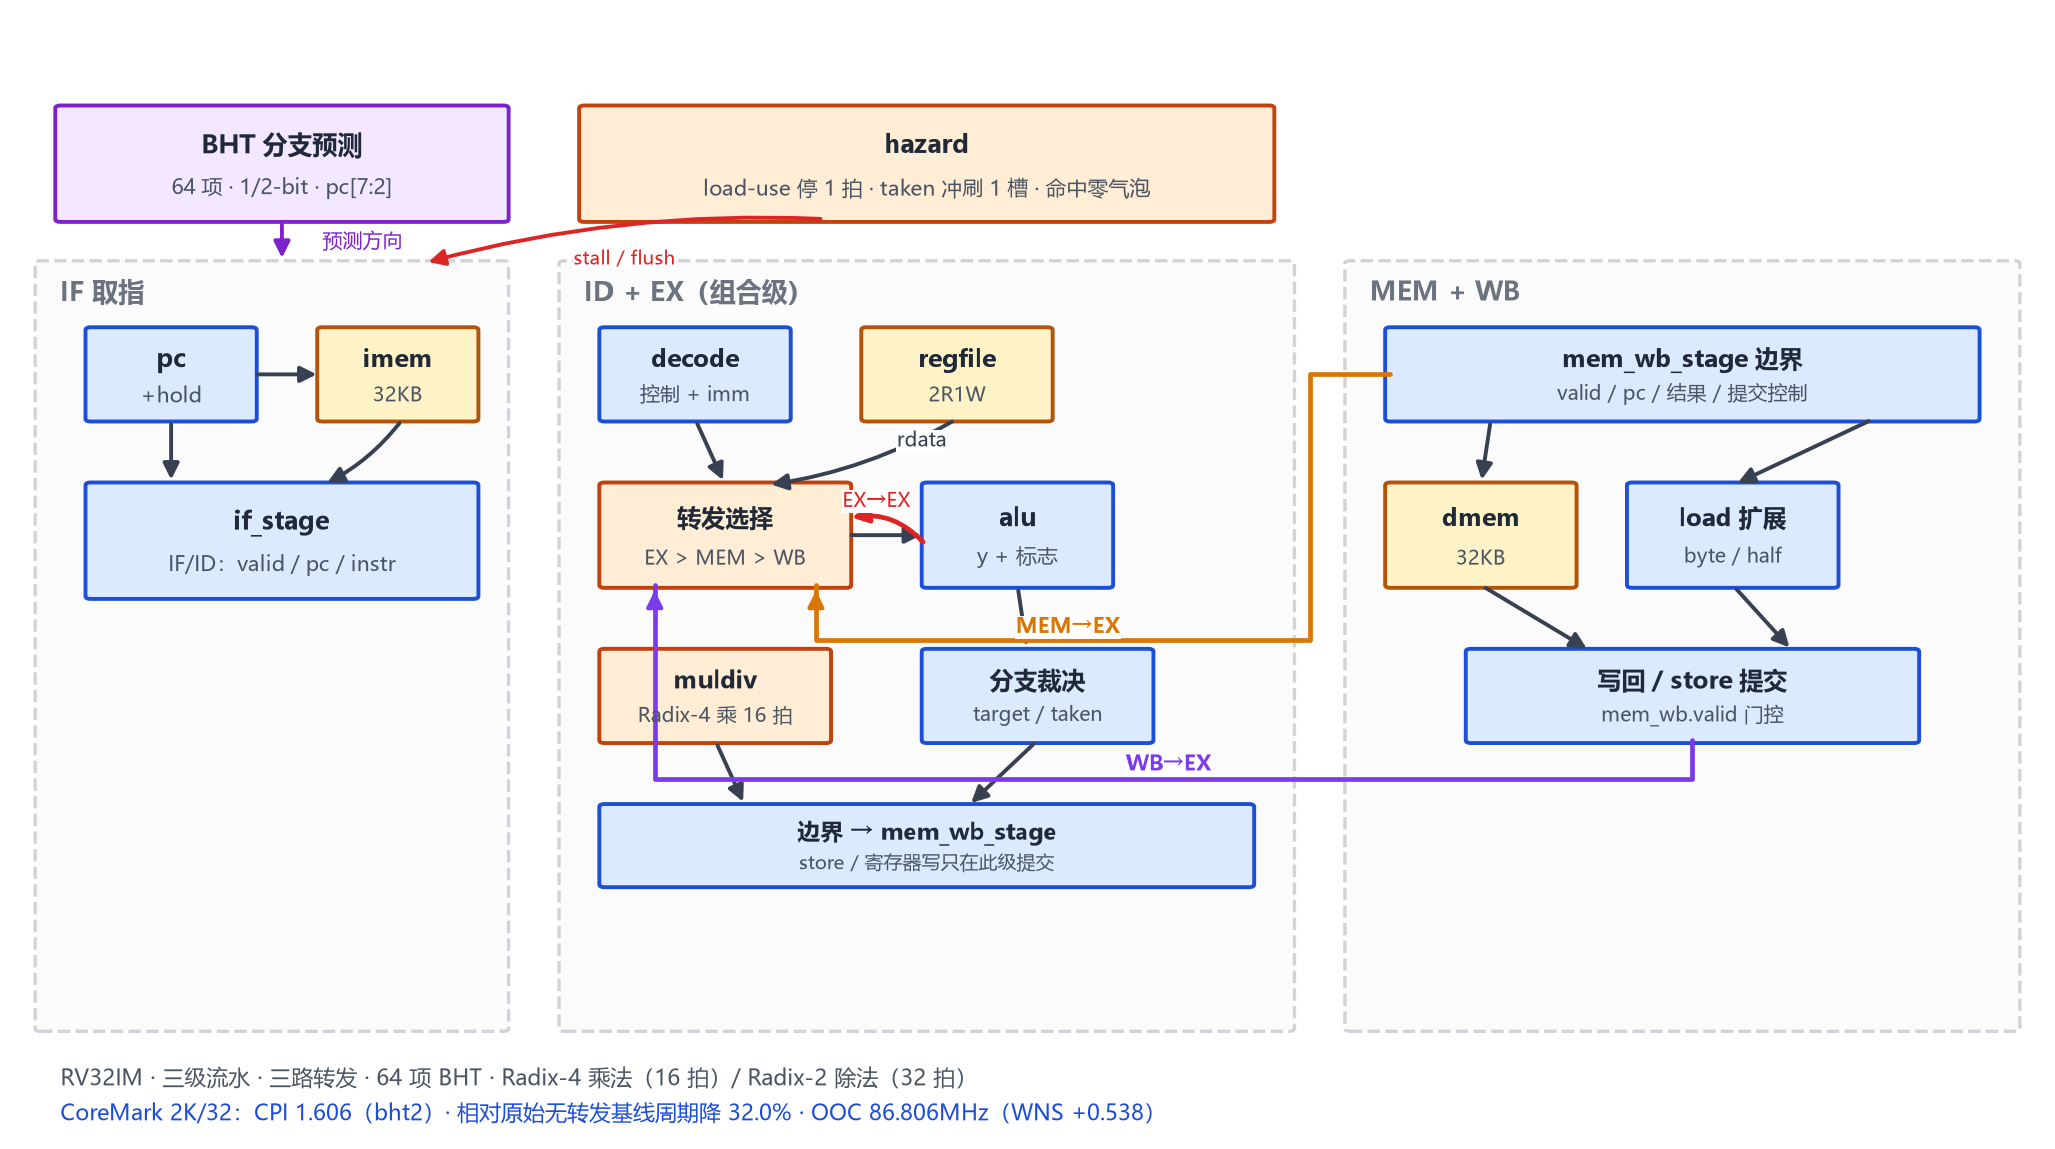
\includegraphics[width=0.98\linewidth]{fig_core.png}
\caption{RISC-V 三级流水、三路转发与 BHT（仓库配图）}\label{fig:core}
\end{figure}

\subsection{微架构}
v1 核为三级流水（IF/ID、EX/MEM、MEM/WB），三路转发优先级为 EX、MEM、WB、寄存器堆。
乘除法采用 Radix-4 基四乘法（16 次迭代）与 32 拍恢复除法，除零与 \code{INT_MIN/-1} 边界显式处理。
分支预测为 64 项 BHT，支持 1-bit 与 2-bit 两档，可经参数切换。
对照档为同一份 RTL 的参数开关，不维护第二份代码。

\subsection{性能：CoreMark 与分类记账}
CoreMark 统一 2K/32 iterations、-O2、统一退休口径；结果为仿真外推值，非官方认证分数。
四档数据见表~\ref{tab:coremark}。

\begin{table}[H]\centering\small
\caption{CoreMark 四档（retired 10{,}106{,}386 条指令）}\label{tab:coremark}
\begin{tabularx}{\linewidth}{@{}P{42mm}P{30mm}Y@{}}\toprule
配置 & CPI & CoreMark/MHz\\\midrule
v0 两级（外部锚点） & 2.105 & 1.506\\
v1 三级，无转发 & 1.886 & 1.681\\
v1 三级，转发 & 1.693 & 1.872\\
v1 三级，转发+BHT1 & 1.616 & 1.961\\
v1 三级，转发+BHT2 & 1.606 & 1.974\\\bottomrule
\end{tabularx}\end{table}

性能收益按优化项分类记账，不混记：固定 Radix-4 乘法器后开关转发，CPI 降幅 10.20\%；固定转发后更换乘法器，周期降幅 21.95\%；两项相对原始无转发基线的组合降幅 28.30\%；转发基础上启用 BHT2 再降 5.15\%。
25\% 为组合优化的尽力目标，未作为单一手段的门禁；原始 FAIL 数据永久保留。

\subsection{功能验证}
riscv-arch-test 以官方 golden 签名为判据：I+M 子集 44/44 签名匹配，档间签名一致。
官方 \code{beq-01} 用例超出 32 KB 链接上限（溢出 195{,}388 字节），故采用 3I+8M 子集，失败留证。
CoreMark 结果与宿主机 -O2、-O0 双档交叉核对，CRC 三方一致。
回归入口为 \code{sim/scripts/run_iverilog.sh}，tb 全部位于仓库内。

\subsection{时序与上板}
时序采用外推、实点、板上三档口径：\code{@10 ns} 约束下仅无转发档通过（WNS +0.051 ns）；BHT2 以 11.52 ns 独立约束实点通过，WNS +0.538 ns，对应 86.806 MHz（表~\ref{tab:coretiming}）。

\begin{table}[H]\centering\small
\caption{核 OOC 时序口径（WNS，ns）}\label{tab:coretiming}
\begin{tabularx}{\linewidth}{@{}P{46mm}P{26mm}Y@{}}\toprule
配置与约束 & WNS & 结论\\\midrule
v1 无转发 @ 10 ns & +0.051 & 通过\\
v1 转发 @ 10 ns & $-0.587$ & 未通过，留档\\
v1 转发+BHT1 @ 10 ns & $-0.419$ & 未通过，留档\\
v1 转发+BHT2 @ 10 ns & $-0.586$ & 未通过，留档\\
v1 转发+BHT2 @ 11.52 ns & +0.538 & 通过，实点 86.806 MHz\\\bottomrule
\end{tabularx}\end{table}

最小 SoC（核 + 32 KB 哈佛存储 + LED 外设）以 40 MHz 上板，WNS +3.618 ns，LUT 6{,}768、FF 859、BRAM 8、DSP 0，LED 显示与固件预期一致。
SoC 125 MHz 构建 WNS $-8.044$ ns，FAIL 记录保留，不作为当前能力声明。
\FloatBarrier

\Needspace{10\baselineskip}
\section{HDMI 视觉预处理流水线}
\label{sec:vision}
视觉预处理流水线为全自研 Verilog-2001 RTL，目标 720p60，流水线结构见图~\ref{fig:video}。

\begin{figure}[H]\centering
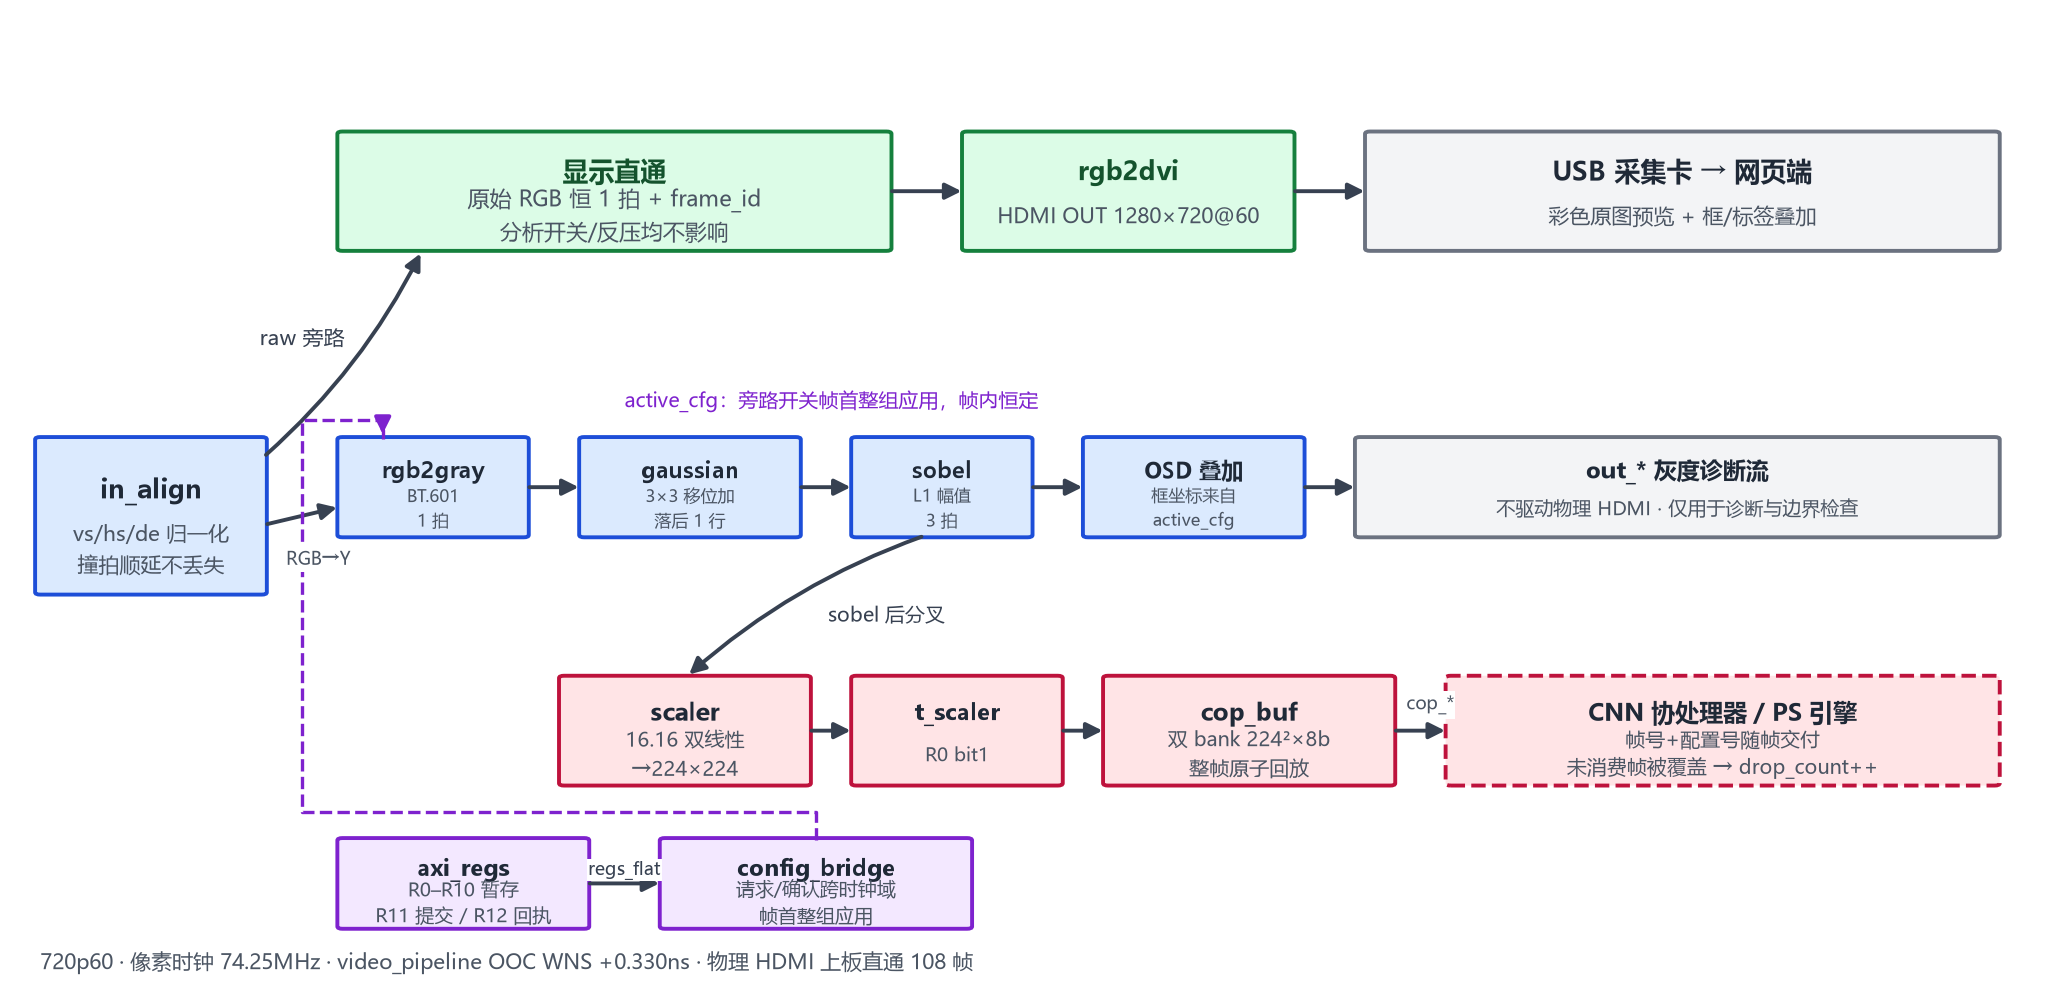
\includegraphics[width=0.98\linewidth]{fig_video.png}
\caption{视觉流水线三路径：显示直通、灰度分析与快照推理（仓库配图）}\label{fig:video}
\end{figure}

\subsection{流水线组成}
链路为 HDMI 接收（\code{dvi2rgb}）、输入对齐、高斯滤波、Sobel 边缘、缩放（scaler）与乒乓缓冲（\code{cop_buf}）。
配置寄存器采用原子配置契约：配置项成组提交、成组生效，避免运行中半新半旧的中间状态。
板上未搭载 ADV7611 器件，HDMI 接收采用 \code{dvi2rgb}/\code{rgb2dvi} 方案。

\subsection{显示与分析分流}
视频与分析路径在 RTL 内分流：
彩色原图以恒定延迟直通 \code{display_*} 口，用于 HDMI OUT 显示，保留原始色彩；
分析路径独立输出灰度 \code{out_*} 口，供定位与推理使用，坐标映射回显示画面。
该分流保证显示帧率不受分析耗时影响，也保证分析用的像素与训练采集的像素同源。

\subsection{时序收敛}
各单元 OOC 综合结果见表~\ref{tab:visiontiming}。
scaler 初版 57.5 MHz 的主因为 lerp 乘法的 9 级进位链；切拍重排读调度后达 94.9 MHz，720p60 全链正裕量。
\code{video_pipeline} 整体 OOC WNS +0.330 ns（2026-10-27 口径）。

\begin{table}[H]\centering\small
\caption{视觉单元 OOC 时序（OOC 综合口径）}\label{tab:visiontiming}
\begin{tabularx}{\linewidth}{@{}P{40mm}P{34mm}Y@{}}\toprule
单元 & 频率口径 & 备注\\\midrule
处理单元 & 约 88 MHz & 初版 OOC\\
高斯/Sobel & 约 76 MHz & 初版 OOC\\
scaler（初版） & 57.5 MHz & lerp 乘法进位链\\
scaler（切拍重排后） & 94.9 MHz & 720p60 全链正裕量\\
\code{video_pipeline} 整体 & WNS +0.330 ns & 2026-10-27 口径\\\bottomrule
\end{tabularx}\end{table}

\subsection{验证}
视觉 RTL 配有 22 个仓库内 tb（2026-10-27 口径），当前脚本入口以 \code{sim/scripts} 为准。
六套黄金参考与 RTL 输出逐像素对拍，误差不超过 2 LSB。
XSim 与 Icarus 双工具对拍，交叉排除仿真器差异。
物理 HDMI 板级直通实测 108 帧稳定输出（2026-10-03 上板记录）。
数据采集规程规定数据集必须经板卡 \code{hdmi_in.readframe()} 采集，保证数据集像素与部署像素一致。
\FloatBarrier

\clearpage
\Needspace{10\baselineskip}
\section{CNN 推理协处理器}
\label{sec:cop}
协处理器执行紧固件分类网络的 INT8 推理，数据通路与寄存器接口见图~\ref{fig:cop}。
整数语义由 C02 契约冻结（表~\ref{tab:c02}），集成分工由 C03 契约冻结。

\begin{figure}[H]\centering
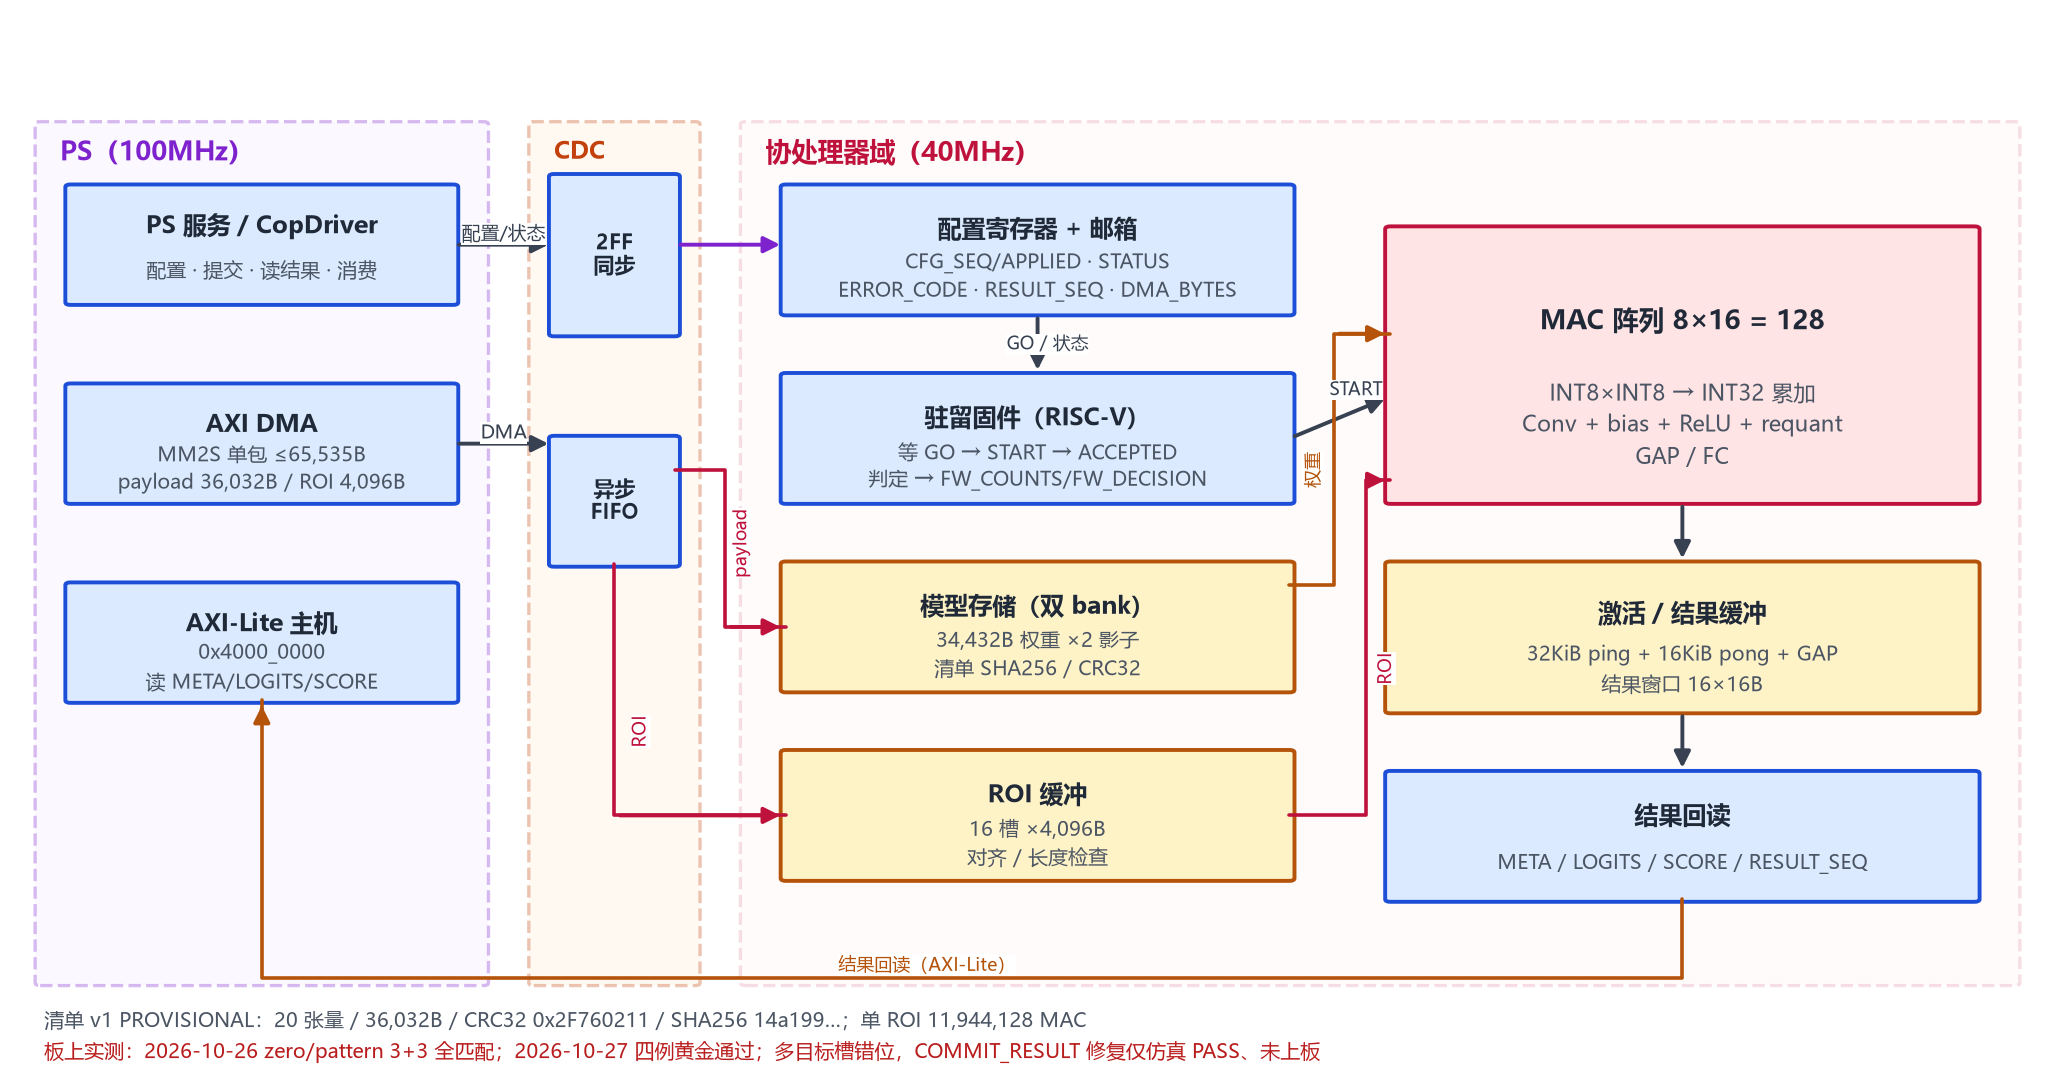
\includegraphics[width=0.98\linewidth]{fig_cop.png}
\caption{CNN 协处理器数据通路、寄存器与 DMA（仓库配图）}\label{fig:cop}
\end{figure}

\begin{table}[H]\centering\small
\caption{C02 整数契约要点}\label{tab:c02}
\begin{tabularx}{\linewidth}{@{}P{34mm}Y@{}}\toprule
项目 & 约定\\\midrule
输入 & 64$\times$64 灰度 ROI\\
权重量化 & per-channel 对称 INT8\\
激活量化 & per-tensor INT8\\
累加 & INT32\\
再量化 & multiplier + 右移 + 饱和\\
计算阵列 & 128 MAC（8$\times$16），100 MHz\\
结果语义 & 并列时取较小类别；\code{score_q15} 线性映射裕度\\\bottomrule
\end{tabularx}\end{table}

\subsection{微架构与优化}
整网控制器调度卷积、偏置、ReLU、再量化、全局平均池化与全连接。
初版综合 WNS $-19.892$ ns，经分拍重整后收敛至 +0.058 ns（192 DSP）。
快速模式重排发射调度后：整网 1{,}123{,}109 拍降至 472{,}593 拍，DSP 192$\rightarrow$136，LUT 10{,}100$\rightarrow$4{,}540。
权重存储采用 16 路 64-bit bank 的真实读延迟 BRAM，每发射拍 136 字节；容量与端口带宽分别核算，不以容量替代端口验证。

\subsection{生产与消费握手}
任务握手语义：PS 独占 \code{CONSUME} 清终态；\code{ACCEPTED} 粘滞；\code{RESULT_SEQ} 单调递增。
固件按\emph{校验序号、落盘成功、再消费}的顺序处理，宁可停顿不以丢数据换流畅。
固件 \code{cop_job.c} 为 52 行 RV32I 代码，与主机共用判定头文件。
看门狗覆盖 \code{NO_ACK}、硬件超时与过期结果三类异常。

\subsection{板级集成与门禁}
板级集成的关键决策：
DMA 描述符长度位宽由 14 位扩至 16 位，36{,}032 字节负载单笔传输，禁止分包（每笔 DMA 产生 TLAST）；
加载器 fail-closed，manifest、SHA256、CRC32 与 HWH 四重校验不过即拒绝；
IMEM 初值设四重门禁（绝对路径、首字校验、RAMB INIT 回读、综合日志扫描），杜绝位流不带固件的假通过；
时钟采用片内 MMCM 产生 40 MHz 并由 HWH 绑定核对，PS 直供方案曾被时钟门禁拦截（实测 142.857 MHz）。
整机门禁的演进见表~\ref{tab:wholegate}。
整机（非 OOC）门禁断言 WNS$\geq$0、DSP$\leq$220、BRAM36$\leq$140、check\_timing 四项为零、DRC 为零、锁存器为零、CDC 例外清单 fail-closed；部件 OOC 资源相加不得冒充整机结果。

\begin{table}[H]\centering\small
\caption{整机门禁演进（40 MHz 整机构建）}\label{tab:wholegate}
\begin{tabularx}{\linewidth}{@{}P{34mm}P{30mm}Y@{}}\toprule
构建 & WNS & 说明\\\midrule
2026-10-22 首过 & +2.498 ns & 修复资源超限与未约束端点后\\
2026-10-26 边沿修复版 & +3.062 ns & DSP 136、BRAM36 69\\
2026-10-27 A 包 & +2.078 ns & 116/116 文件校验，随核共存\\\bottomrule
\end{tabularx}\end{table}

\subsection{板上验证}
2026-10-26，协处理器首次获得实板硬件 CNN 输出：zero 与 pattern 诊断网各 3 轮，6/6 与预期一致。
随后四例黄金（zero、pattern、\code{roi_001}、frame）全部匹配，寄存器 10{,}000 次连续读取无错误。
共存位流同时输出 HDMI、抓取 BGR 原帧并运行硬件 CNN。
2026-10-28，多目标修复包上板：CNN r6 两组真实 ROI 共 12 轮 85 个结果，logits、类别、有效位与裕度同整数参考逐项一致，结果槽错位未再出现（WNS 1.359 ns 位流）。
以上为单目标与多目标推理正确性证据；识别精度见第~\ref{sec:data} 节的边界说明。
\FloatBarrier

\Needspace{10\baselineskip}
\section{数据、模型与工业闭环}
\label{sec:data}
本章说明数据采集、模型训练与量化、检查语义与前端形态。

\subsection{数据采集与审计}
数据集必须经板卡 \code{hdmi_in.readframe()} 采集，保证数据集像素与部署像素一致。
数据集实行清单化管理：来源、格式、训练/测试泄漏、空场景与实物分层审计，防泄漏审计含会话与实物双维划分及双哈希核对，共 13 组回归。
软件分层与一次检查的作业时序见图~\ref{fig:sw}。

\begin{figure}[H]\centering
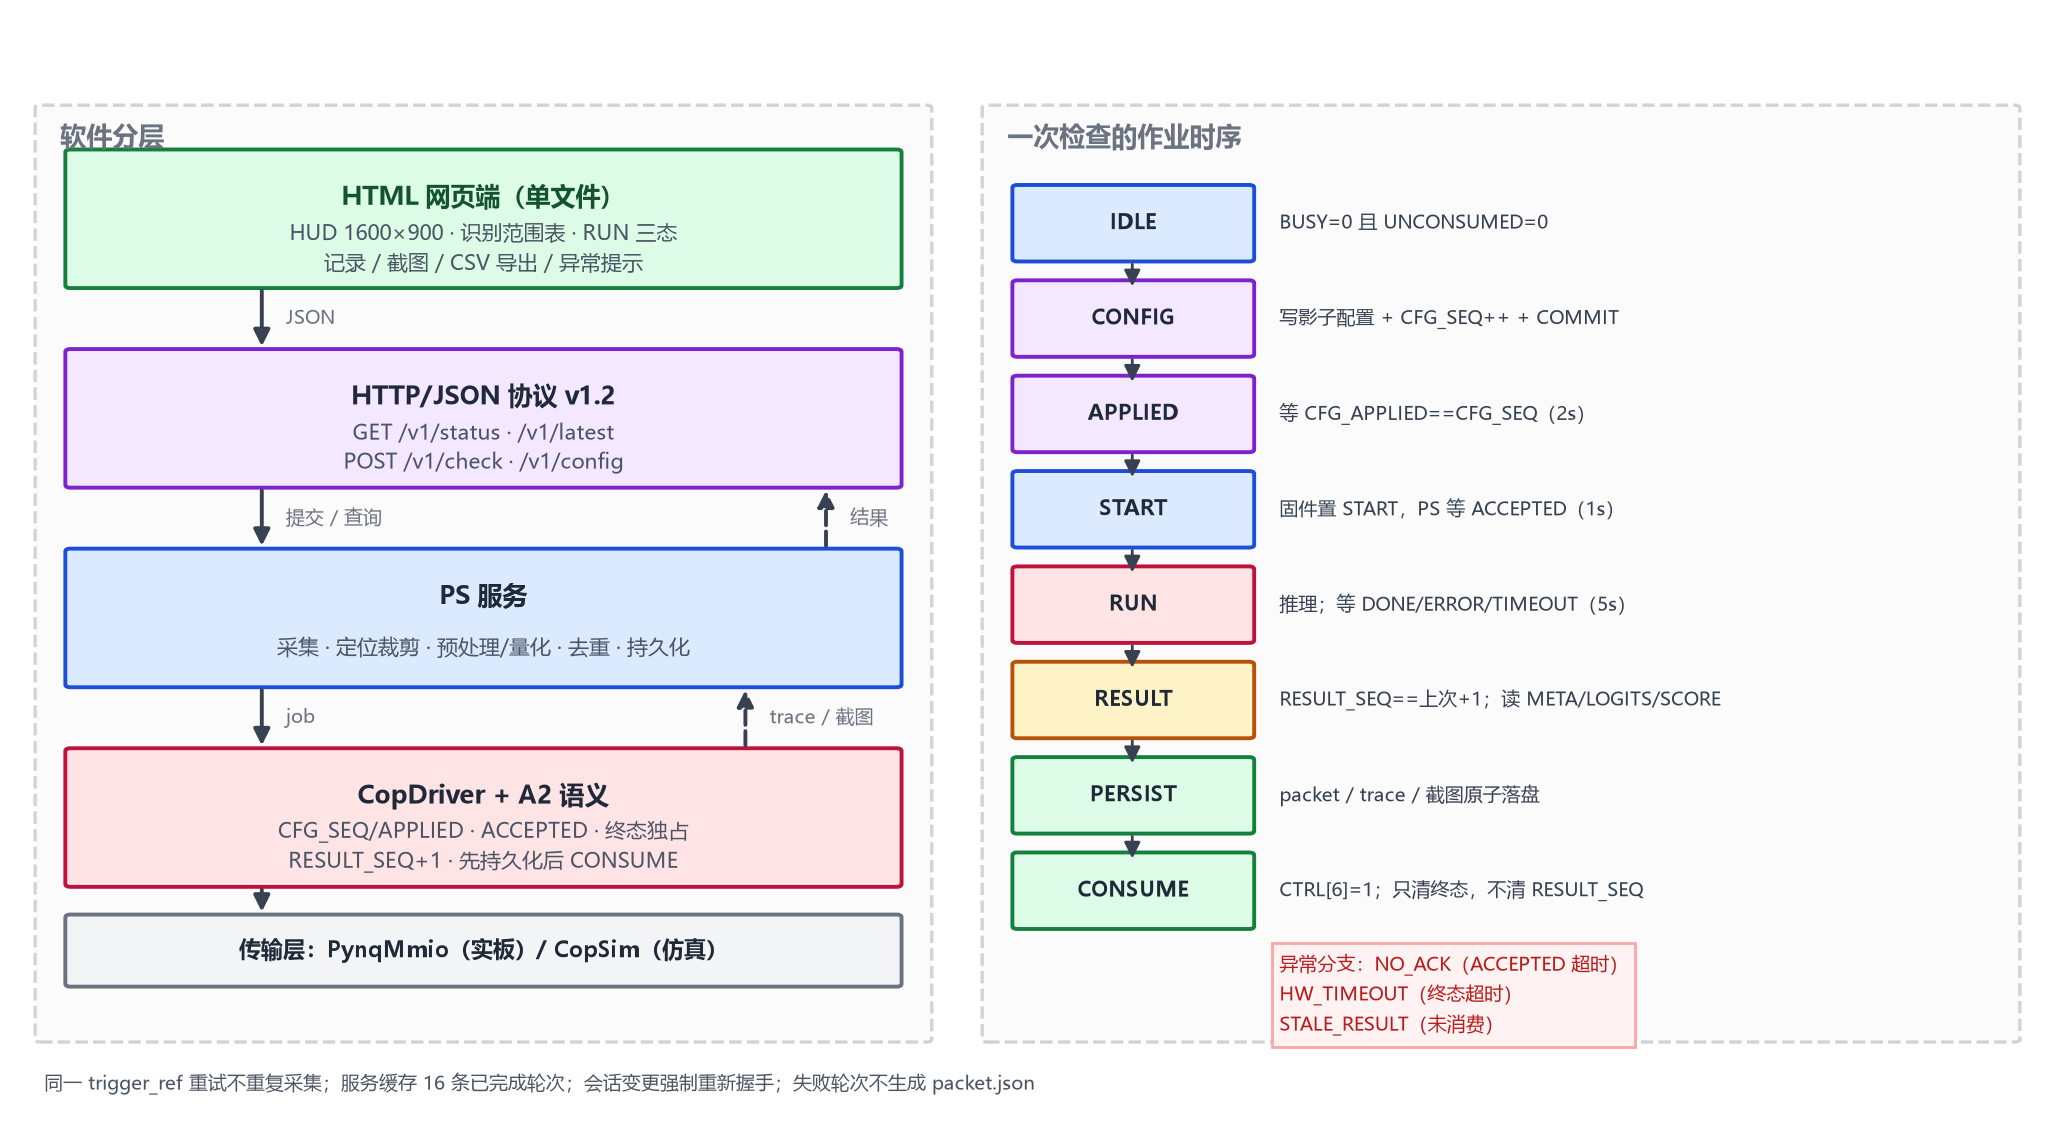
\includegraphics[width=0.98\linewidth]{fig_sw.png}
\caption{软件分层与一次检查的作业时序（仓库配图）}\label{fig:sw}
\end{figure}

\subsection{模型与量化}
分类网络为 64$\times$64 灰度小模型，按 C02 契约做训练后量化（PTQ）。
当前工作版本 r6：训练集 33 个 ROI，训练拟合与 PTQ 校准分类一致均为 33/33；未参与训练的清晰 5 螺母图 FP32 与 INT8 均为 5/5（含竖立螺母）。
权重、参数与复现命令见 CNN r6 证据包。

\subsection{留出对照与边界}
新摆放留出图（9 件，未参与训练与校准）对照结果见表~\ref{tab:holdout}。
全部 9 件被定位；FP32 与 INT8 各正确 8/9，均将 3 号垫圈判为螺母；分类一致性 9/9。
另有混合摆放 10 件图，定位与分类视觉复核 10/10，但未逐编号确认。
上述均为同工位开发对照，不是正式独立精度验收；换实物、换环境的泛化验收未实现，分类一致不能替代分类正确。

\begin{table}[H]\centering\small
\caption{CNN r6 留出摆放对照（9 件）}\label{tab:holdout}
\begin{tabularx}{\linewidth}{@{}P{42mm}P{30mm}Y@{}}\toprule
项目 & 结果 & 说明\\\midrule
定位 & 9/9 & 全部出框\\
FP32 分类正确 & 8/9 & 3 号垫圈判为螺母\\
INT8 分类正确 & 8/9 & 同上\\
分类一致性（FP32 vs INT8） & 9/9 & 不代表分类正确\\\bottomrule
\end{tabularx}\end{table}

\subsection{检查语义与记录}
检查按工单核对类别与数量，输出缺件、多余件、错料与复检提示。
重复帧不增加批次计数：记录资格绑定手动触发，属结构性保证。
异常事件附截图入档；记录导出为 UTF-8 BOM 的 CSV，避免 Excel 乱码。
断联、过期或无法确认的画面不显示为当前检查通过。

\subsection{前端形态}
前端为 HTML 网页端（\code{src/web_client}），经本机 Python 服务转发到板端，页面不直接访问硬件。
网页端已接入真实采集卡视频与板端轮次（2026-10-30 联调、2026-11-03 实验室复测）：
页面填写并下发工单（各类 0--10 件、合计 1--10 件），板端校验回显后配置号递增，未应用时禁止开始检查；
结果按接收时刻计龄 4.5\,s，超龄、断联或配置不符立即撤框；自动轮询默认暂停、单请求在途；
手动有效轮次按会话与检查编号去重，记录导出为 UTF-8 BOM 的 CSV。
当前按单页使用：同会话的第二个客户端会争用配置并导致连接中断，属已知限制。
桌面程序已于 2026-10-28 全套退役，历史记录保留在 git 历史与当日协作日志中。
\FloatBarrier

\clearpage
\Needspace{10\baselineskip}
\section{完成情况与验收边界}
\label{sec:status}
本章按三态口径盘点完成度：已实现并验证、已实现未验证、未实现。
口径以主计划（2026-10-28）与三态盘点（2026-10-26）为准。

\subsection{完成度矩阵}
完成度矩阵见表~\ref{tab:status}。
\begin{table}[H]\centering\small
\caption{完成度矩阵（三态口径，含口径日期）}\label{tab:status}
\begin{tabularx}{\linewidth}{@{}P{14mm}Y@{}}\toprule
状态 & 事项\\\midrule
已实现并验证 & 核与最小 SoC 收口（2026-10-07）；视觉 RTL 与真实视频链路；视觉 RTL tb、视觉 Python 与 INT8 参考测试全量回归；FILE/LIVE 原型与前端展示离板验证；网页端真机联调（2026-10-30 联调、2026-11-03 工单下发与 CSV 导出复测）；板上硬件 CNN 四例黄金与 10{,}000 次寄存器读取（2026-10-26/27）；多目标 12 轮 85 结果与整数参考一致（2026-10-28）；CNN r6 训练与校准 33/33（2026-10-28）\\
已实现未验证 & 含 DMA 边沿修复的早期位流与 trained 包（构建完成，当时未上板；多目标修复已随 2026-10-28 共存位流上板）；正式工位构图与拍摄条件；网页端连续多轮稳定性（2026-10-30 同会话第 5 轮出现任务错误、随后 DMA 超时，根因未定位）\\
未实现 & 全链整机验收；正式 INT8 模型与生产黄金；换实物泛化验收；工位实测矩阵（N10--N12）；连续运动的触发、关联与去重\\\bottomrule
\end{tabularx}\end{table}

\subsection{结果讨论}
核与协处理器的正确性证据链完整：架构测试签名、CoreMark 交叉核对、量化逐位黄金、板上黄金对照逐级覆盖。
推理正确性与识别精度是两件事：黄金对照证明整数链与硬件输出一致，不证明识别精度；留出图对照给出诚实的精度快照（8/9），正式精度报告待真实数据与正式工位。
工单判定与记录链路经离板与软件联调验证；网页端已接入真实视频流、板端服务与记录导出，并完成页面工单下发；
连续多轮稳定性未验收，故整机验收不能宣称完成。

\subsection{验收边界声明}
本报告区分四级证据：离板仿真、软件联调、单目标板上推理、整机验收。
PROVISIONAL 黄金对拍不等同于识别精度，也不等同于整机验收。
性能指标均为实测留档口径，外推值单独标注。
\FloatBarrier

\Needspace{10\baselineskip}
\section{总结与可扩展之处}
\label{sec:conclusion}

\subsection{总结}
项目在一块 PYNQ-Z2 上完成三个自研数字模块的协同：视觉预处理流水线、INT8 CNN 协处理器与自研 RISC-V 核，并配套 PS 服务与网页前端。
工程质量依赖四项制度：契约先行、逐位黄金对拍、理解门槛入库、证据目录留痕。
每一项对外声称的能力都能由仓库内脚本复现；每一项未完成的能力都在主计划与三态盘点中如实登记。

\subsection{可扩展之处}
模型侧：更多类别与更大的网络，量化感知训练（QAT）替代 PTQ，正式工位下的精度报告。
架构侧：目标定位由 PS 下沉至 PL，减少 DDR 往返；协处理器支持多任务连续作业，减少每任务重配置。
应用侧：连续运动场景的触发、关联与去重；跨帧跟踪与更多工单语义；温度与长时稳定性测试。
流程侧：网页端三项接线完成后，即可开展全链整机验收与现场演示。

\clearpage
\appendix
\Needspace{10\baselineskip}
\section{附录}
\label{sec:appendix}

\subsection{复现入口}
复现入口见表~\ref{tab:repro}。
\begin{table}[H]\centering\small
\caption{仓库内复现入口}\label{tab:repro}
\begin{tabularx}{\linewidth}{@{}P{68mm}Y@{}}\toprule
入口 & 覆盖范围\\\midrule
\code{bash sim/scripts/run_iverilog.sh all} & RTL 全量回归（核、视觉、协处理器 tb）\\
\code{python sim/scripts/check_repo_hygiene.py} & 仓库卫生门禁（预算、断链、生成物）\\
\code{data/logs/<日期-主题>/README.md} & 实验证据目录（命令、结果、产物、边界）\\
\code{data/evidence/<日期-主题>/README.md} & 权重、位流等大件证据与复现命令\\
\code{report/llm_log/} & 大模型协作记录与理解门槛落盘\\
\code{docs/runbooks/} & 板端交接与复现手册\\\bottomrule
\end{tabularx}\end{table}

\subsection{术语表}
常用术语见表~\ref{tab:terms}。
\begin{table}[H]\centering\small
\caption{术语表}\label{tab:terms}
\begin{tabularx}{\linewidth}{@{}P{30mm}Y@{}}\toprule
术语 & 含义\\\midrule
PL / PS & FPGA 可编程逻辑 / Zynq 处理系统\\
OOC & Out-of-Context 综合，单元级时序与资源口径\\
WNS / WHS & 建立时间 / 保持时间最差裕量\\
CPI & 每指令周期数\\
BHT & 分支历史表（分支预测）\\
arch-test & riscv-arch-test 官方架构测试（签名比对）\\
黄金参考 & 独立于被测实现的参考输出，用于逐位对拍\\
三态口径 & 离板仿真 / 综合（门禁）/ 板上（实测）三级标注\\
PTQ & 训练后量化\\
ROI & 感兴趣区域（目标裁剪框）\\
MMIO / AXI4-Lite & 内存映射寄存器 / 轻量总线接口\\
DMA & 直接内存访问\\
CDC & 跨时钟域\\
PROVISIONAL & 临时口径数据，未达正式发布条件\\
UNVERIFIED & 已构建但未获板级实测证据\\
park 驱动 & 借助暖机窗口完成 DDR 帧复制的取帧方案\\
轮次协议 v1.2 & 视频、结果与检查轮次的关联契约（16 目标上限）\\
C01--C04 & DDR 帧所有权 / 整数契约 / 集成契约 / 应用语义四份冻结契约\\
理解门槛 & AI 生成代码入库前的讲解与测试制度\\\bottomrule
\end{tabularx}\end{table}

\subsection{素材清单}
图片素材与状态见表~\ref{tab:materials}。
\begin{table}[H]\centering\small
\caption{图片素材与状态}\label{tab:materials}
\begin{tabularx}{\linewidth}{@{}P{34mm}Y@{}}\toprule
素材 & 状态\\\midrule
\code{fig_system.png}、\code{fig_video.png}、\code{fig_core.png}、\code{fig_cop.png}、\code{fig_sw.png}、\code{fig_flow.png} & 已入库（\code{docs/tech-report/figures/}）\\
\code{photo_plate.jpg} 等实物照片 & 已入库\\
网页端实机运行截图 & 待补充（桌面程序已退役，需新形态截图）\\
团队与成员信息 & 待补充\\
\bottomrule
\end{tabularx}\end{table}
\FloatBarrier

\begin{thebibliography}{9}
\bibitem{plan}\sourcepath{plan.md}{项目主计划（2026-10-28 口径）}，2026-10-28。
\bibitem{m1closure}\sourcepath{report/module1-closure.md}{模块一核与最小 SoC 收口报告}，2026-10-07。
\bibitem{designv1}\sourcepath{src/riscv/design_v1.md}{RISC-V v1 冻结契约（含 \S 14.2 性能口径）}。
\bibitem{cpi}\sourcepath{data/logs/2026-10-05-partB-v1-coremark-cpi/}{转发双档 CoreMark 原始数据}，2026-10-05。
\bibitem{radix4}\sourcepath{data/logs/2026-10-05-partB-radix4-cycle-breakdown/}{Radix-4 乘法器周期分解}，2026-10-05。
\bibitem{visionoff}\sourcepath{data/logs/2026-10-02-vision-offboard/}{视觉预处理离板收口}，2026-10-02。
\bibitem{visionon}\sourcepath{data/logs/2026-10-03-vision-onboard/}{视觉链路上板记录}，2026-10-03。
\bibitem{c02}\sourcepath{src/coprocessor/design_v0.md}{C02 协处理器整数契约}。
\bibitem{c03}\sourcepath{docs/contracts/coprocessor-integration-v0.md}{C03 集成契约（MMIO/AXI4-Lite + DMA）}。
\bibitem{sync}\sourcepath{docs/contracts/vision-sync-protocol-decisions.md}{视觉轮次协议 v1.2 裁决记录}。
\bibitem{r6board}\sourcepath{data/logs/2026-10-28-multitarget-board-r6/}{多目标修复与 r6 实板数值对照}，2026-10-28。
\bibitem{r6pkg}\sourcepath{data/evidence/2026-10-28-cnn-r6/}{CNN r6 权重、参数与复现命令}，2026-10-28。
\bibitem{status26}\sourcepath{report/project-final-status-2026-10-26.md}{项目三态盘点（只记录事实）}，2026-10-26。
\bibitem{coexist}\sourcepath{docs/runbooks/pynq-coexist-handoff-2026-10-27.md}{PYNQ 共存位流交接单}，2026-10-27。
\bibitem{llmlog}\sourcepath{report/llm_log/}{大模型协作记录（218 篇）}，2026-09-04 至 2026-10-29。
\end{thebibliography}
\end{document}
